\chapter{Fluoride Adsorption Optimization Using GTMAC-Modified Coconut Fiber and Machine Learning}
 Fluoride contamination in drinking water is a major environmental concern due to its harmful health effects. The need for low-cost and eco-friendly fluoride removal methods has increased interest in biomass-based adsorbents such as coconut fiber. In the present work, coconut fiber is modified using Glycidyl Trimethyl Ammonium Chloride (GTMAC) to improve fluoride adsorption characteristics. Design of Experiments (\gls{doe}) using Central Composite Design (\gls{ccd}) is used for planning adsorption studies and optimization. This chapter presents the background, literature review, objectives, methodology, and organization of the report related to the study. 

\section[Introduction]{\textbf{Introduction}}
These Fluoride contamination in drinking water is a major environmental and public health issue, especially in groundwater sources where fluoride levels may exceed the WHO permissible limit of 1.5 mg/L. Excess fluoride intake can cause dental and skeletal fluorosis, making effective defluoridation essential. Conventional treatment methods such as reverse osmosis, ion exchange, and activated alumina are efficient but often expensive and difficult to implement in small-scale or decentralized systems. Therefore, low-cost and sustainable biomass-based adsorbents have gained attention for water purification applications. Coconut fibre is an abundant agricultural waste material containing cellulose and lignin, but its natural fluoride adsorption capacity is limited due to the lack of sufficient active adsorption sites. 

In this project, coconut fibre is chemically modified using Glycidyl Trimethyl Ammonium Chloride (GTMAC) to improve its fluoride adsorption performance by introducing positively charged quaternary ammonium groups on the surface. Batch adsorption studies are carried out using Design of Experiments (\gls{doe}) and Central Composite Design (\gls{ccd}) to analyse the effect of important parameters such as pH, adsorbent dose, initial fluoride concentration, and contact time through multiple experimental runs. The study also incorporates Langmuir isotherm modelling and machine learning-based prediction to enhance adsorption analysis and optimize fluoride removal efficiency. This integrated approach combines sustainable material development, statistical optimization, and predictive modelling for efficient fluoride removal from water. 

\begin{figure}[H]
	\centering
	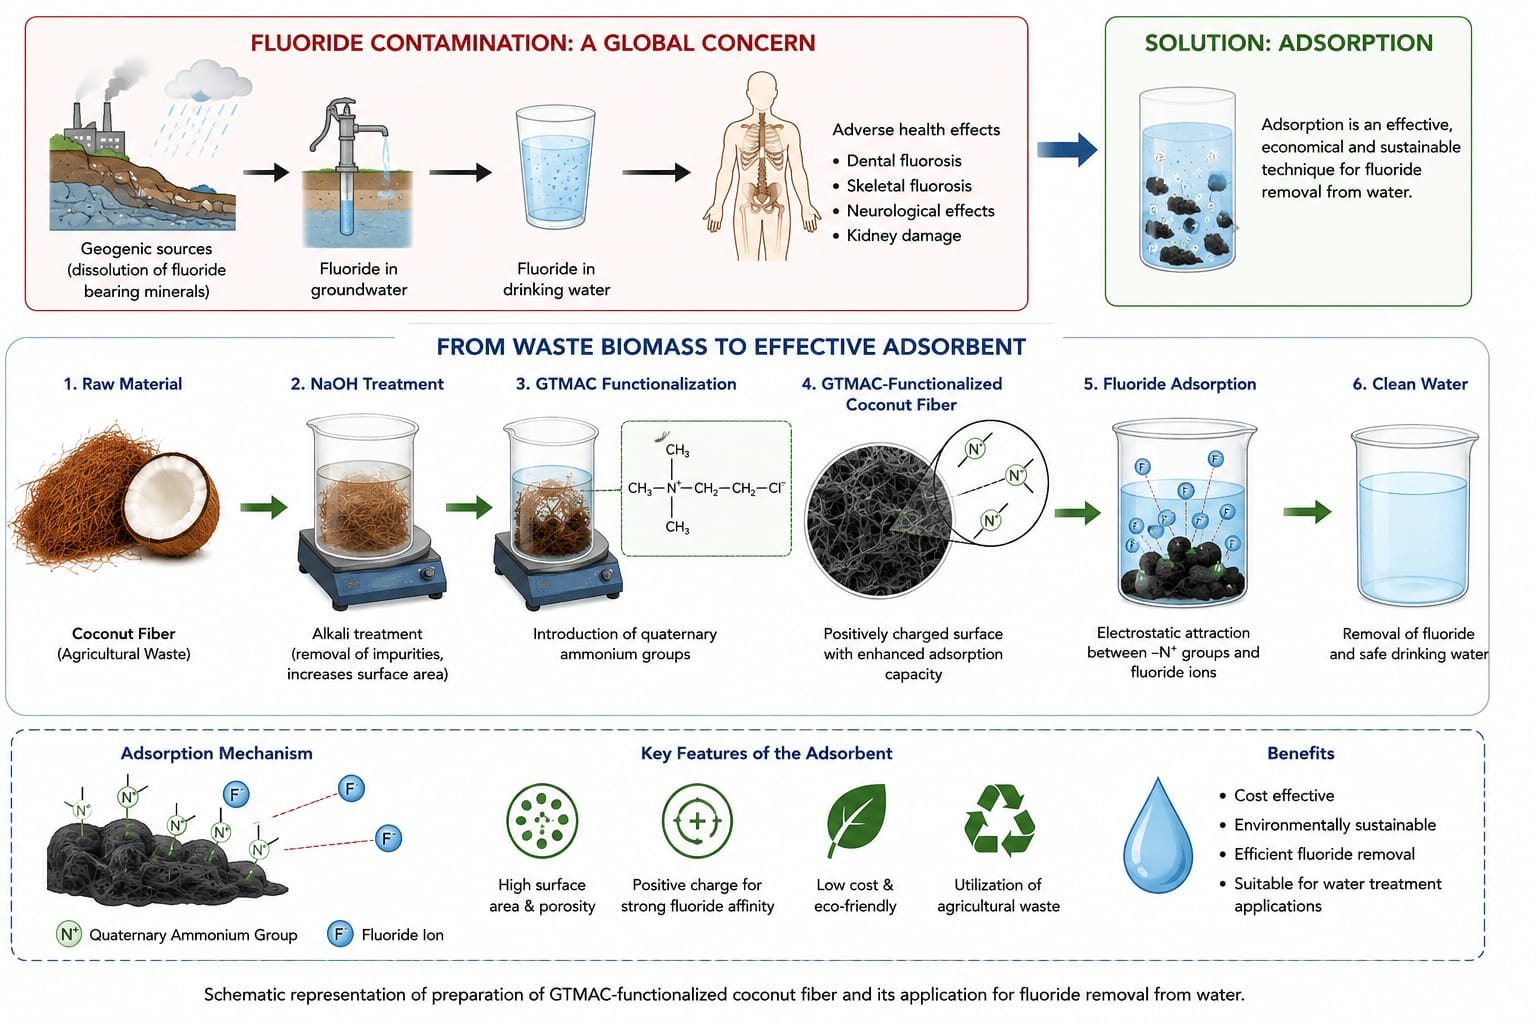
\includegraphics[width=0.7\textwidth]{Chapter1/Figures/1.jpeg}
	\caption{Schematic representation of preparation, functionalization, and application of GTMAC-modified coconut fiber for fluoride removal from water.}
	\label{fig:labelgraphical abstract}
\end{figure}
The schematic illustrates the overall approach adopted for fluoride removal from drinking water using GTMAC-functionalized coconut fiber as a bioadsorbent. The process begins with the utilization of coconut fiber, an agricultural waste biomass, which undergoes alkaline pretreatment using NaOH to remove impurities and activate the cellulose surface. The activated biomass is then functionalized using Glycidyl Trimethylammonium Chloride (GTMAC), introducing positively charged quaternary ammonium groups onto the surface. These functional groups enhance the affinity of the adsorbent toward negatively charged fluoride ions through electrostatic interaction and ion-exchange mechanisms. The modified adsorbent is subsequently applied in batch adsorption studies for fluoride removal from contaminated water. The figure also highlights the environmental and economic advantages of the proposed adsorbent, including low cost, sustainability, and utilization of waste biomass for water treatment applications.



\section[Literature Review]{\textbf{Literature Review}}

 Several researchers have explored the use of low-cost biomaterials for fluoride 
 adsorption from water. Kamilia et al. (2025) reported that GTMAC-modified 
 chitosan-coated magnetic composites exhibited significantly improved adsorption 
 capacity due to the introduction of quaternary ammonium groups \cite{Kamilia2025}. 
 Budeli et al. (2025) demonstrated that tri-metal oxide modified diatomaceous earth 
 achieved nearly 98\% fluoride removal efficiency over a wide pH range \cite{Budeli2025}. 
 Ayalew (2023) studied thermally treated and acid-activated kaolin clay for fluoride 
 adsorption and reported improved adsorption performance after activation \cite{Ayalew2023}. 
 Gogoi et al. (2019) showed that PEI-GTMAC modified biomass adsorbents exhibited 
 enhanced anion adsorption capacity due to increased positive surface charge \cite{Gogoi2019}. 
 Similarly, Chen et al. (2014) explained that GTMAC quaternization increases the density 
 of positively charged functional groups on biopolymers, thereby improving anion adsorption 
 efficiency \cite{Chen2014}. These studies confirm that chemical surface modification plays 
 a major role in improving adsorption performance of biomass materials.
 
 Researchers have also investigated adsorption modelling and optimization techniques for 
 improving fluoride removal efficiency. Mohan et al. (2007) reported that activated alumina 
 follows Langmuir adsorption behaviour and demonstrated strong fluoride affinity through 
 ligand exchange mechanisms \cite{Mohan2007}. Mukherjee et al. (2023) used experimental 
 modelling and parametric optimization for fluoride adsorption studies and highlighted the 
 importance of statistical optimization methods in adsorption research \cite{Mukherjee2023}. 
 Recent studies have also focused on integrating machine learning approaches with conventional 
 adsorption models to improve prediction accuracy under complex operating conditions. The 
 hybrid chemical-machine learning approach combines the physical understanding of adsorption 
 obtained from Langmuir isotherm modelling with the predictive capability of machine learning 
 algorithms for handling nonlinear interactions and residual errors. However, limited work has 
 been reported on GTMAC-functionalized coconut fibre for fluoride removal using \gls{doe} 
 optimization and hybrid predictive modelling \cite{Chauhan2024}. Therefore, the present 
 study focuses on developing a GTMAC-modified coconut fibre adsorbent, optimizing process 
 parameters using Central Composite Design (\gls{ccd}), and integrating Langmuir--Machine Learning 
 modelling for improved fluoride adsorption prediction and optimization \cite{Hussain2024}.

 \subsection[Hybrid Langmuir--Machine Learning Modelling]{\textbf{Hybrid Langmuir--Machine Learning Modelling}}

 The integration of physics-based isotherm models with data-driven machine learning
 techniques has emerged as a powerful strategy for improving adsorption prediction
 accuracy beyond what either approach can achieve independently. The Langmuir isotherm
 provides a thermodynamically grounded description of monolayer adsorption on homogeneous
 sites, expressed through the equilibrium adsorption capacity $q_e$ and the Langmuir
 constant $K_L$. However, in practice, real adsorption systems exhibit nonlinear
 interactions, heterogeneous surface effects, and parameter correlations that the
 Langmuir model alone cannot capture, leading to systematic prediction residuals.

 Hybrid modelling frameworks that couple mechanistic models with machine learning have
 been reported across several adsorption and separation contexts. The core idea is to
 use the physics-based model to generate a baseline prediction and then train a
 machine learning algorithm to predict the residual error between the Langmuir
 prediction and the observed data. This residual correction strategy---sometimes
 called \emph{grey-box} or \emph{physics-informed machine learning}---allows the
 combined model to inherit the interpretability and extrapolation properties of the
 mechanistic model while exploiting the flexibility of data-driven methods to learn
 systematic deviations.

 Several ensemble and neural network architectures have been evaluated for such
 residual correction tasks. Random Forest (\gls{rf}) regressors exploit bootstrap
 aggregation and feature importance ranking to capture variable interactions without
 over-fitting to small datasets. Extreme Gradient Boosting (\gls{xgb}) offers
 superior handling of sparse feature spaces through sequential tree construction with
 regularization, making it well-suited to adsorption datasets with correlated input
 variables such as pH, dose, initial concentration, contact time, and temperature.
 Multilayer Perceptron (\gls{mlp}) neural networks add the capacity to approximate
 arbitrary continuous functions, providing a complementary data-driven component when
 residual patterns are smooth and systematic.

 In the context of fluoride adsorption, Latin Hypercube Sampling (\gls{lhs}) has been
 proposed as an efficient design strategy for generating training datasets that span
 the full multi-dimensional factor space, reducing the number of simulations required
 compared to full-factorial designs while maintaining good space-filling properties.
 The hybrid workflow adopted in the present study follows this paradigm: Langmuir
 isotherm parameters are first estimated from experimental \gls{ccd} data, synthetic
 training points are generated via \gls{lhs} over the ten-dimensional factor space,
 Langmuir predictions are computed for each point, and the resulting residuals
 $\varepsilon = q_{\text{exp}} - q_{\text{Langmuir}}$ serve as the regression target
 for the machine learning models. The final hybrid prediction is:
 \begin{equation}
     q_{\text{hybrid}} = q_{\text{Langmuir}} + \hat{\varepsilon}_{\text{ML}}
 \end{equation}
 where $\hat{\varepsilon}_{\text{ML}}$ is the residual predicted by the trained
 machine learning model. This formulation ensures that the hybrid model reduces to
 the Langmuir baseline when the machine learning correction is negligible, preserving
 physical interpretability. The approach is consistent with the broader trend in
 environmental engineering of combining first-principles knowledge with data-driven
 flexibility to achieve robust, generalizable predictions \cite{Hiremath2024}.
 
%\subsection{Sample}
%The main types of literature reviews are: evaluative, exploratory, and instrumental. A fourth type, the systematic review, is often classified separately, but is essentially a literature review focused on a research question, trying to identify, appraise, select and synthesize all high-quality research evidence and arguments relevant to that question. A meta-analysis is typically a systematic review using statistical methods to effectively combine the data used on all selected studies to produce a more reliable result.
%\subsubsection[Review types]{\textbf{Review types}}
%
%The main types of literature reviews are: evaluative, exploratory, and instrumental. A fourth type, the systematic review, is often classified separately, but is essentially a literature review focused on a research question, trying to identify, appraise, select and synthesize all high-quality research evidence and arguments relevant to that question. A meta-analysis is typically a systematic review using statistical methods to effectively combine the data used on all selected studies to produce a more reliable result.
%
%
%\subsubsection[Process and product]{\textbf{Process and product}}
%
%Distinguish between the process of reviewing the literature and a finished work or product known as a literature review. The process of reviewing the literature is often ongoing and informs many aspects of the empirical research project. All of the latest literature should inform a research project. Scholars need to be scanning the literature long after a formal literature review product appears to be completed.
%
%\subsubsection{\textbf{Page limitation}}
%
%A careful literature review is usually 15 to 30 pages and could be longer. The process of reviewing the literature requires different kinds of activities and ways of thinking and link the activities of doing a literature review with Benjamin Bloom’s revised taxonomy of the cognitive domain (ways of thinking: remembering, understanding, applying, analysing, evaluating, and creating).
%
%This section should contain the review of the literature in the past.You should review a minimum of 10 papers from standard reference journals. Kindly avoid local conference papers and papers from predatory journals. Kindly consult with your guide and finalize papers to be considered for review before adding in this section.Report the major observations and findings from each paper in one paragraph in the format given below.
%
%proposed various techniques for adders and multipliers.Add the reference papers to the bibliography section using Jabref and cite it here using the instructions given in further chapters.
%
%
%\subsubsection{\textbf{Plagiarism}}
%
%To use someone else's exact words without quotation marks and appropriate credit, or to use the unique ideas of someone else without acknowledgement, is known as plagiarism. In publishing, plagiarism is illegal; in other circumstances, it is, at the least, unethical. You may quote or paraphrase the words or ideas of another if you document your source. Although you need not enclose the paraphrased material in quotation marks, you must document the source. 
%
%Paraphrased ideas are taken from someone else whether or not the words are identical. Paraphrasing a passage without citing the source is permissible only when the information paraphrased is common knowledge in a field. (Common knowledge refers to historical, scientific, geographical, technical, and other type of information on a topic readily available in handbooks, manuals, atlases and other references). 
%
%\subsubsection{How to add Reference}
%Use \texttt{Jabref} which will help in adding the reference in a separate file, from which one can use \verb|\citep\{\}| command to add reference. A sample, referring to a textbook would look something like this,\cite{Razavi2000}.

\section[Motivation]{\textbf{Motivation}}

Fluoride contamination in drinking water is a major health concern as excess fluoride can cause dental and skeletal fluorosis. Conventional fluoride removal methods are effective but expensive and difficult to implement in decentralized systems. This motivated the use of low-cost and eco-friendly biomass materials such as coconut fiber for adsorption studies. Since natural coconut fiber has limited fluoride adsorption capacity, GTMAC surface modification is used to improve its performance. The project also focuses on optimizing the adsorption process using \gls{doe} and improving prediction accuracy through hybrid Langmuir–Machine Learning modelling. 

\section[Problem statement]{\textbf{Problem statement}}

Coconut fiber is a low-cost biomass adsorbent but exhibits limited fluoride removal in its natural form. While GTMAC modification can enhance adsorption, the influence of interacting process parameters is not systematically optimized. Additionally, conventional models like the Langmuir isotherm have limited predictive accuracy under real conditions. This study addresses these gaps by combining surface modification, \gls{doe}-based optimization, and hybrid Langmuir–machine learning modeling to improve fluoride adsorption and prediction.


\section[Objectives]{\textbf{Objectives}}
The objectives of the project are
\begin{enumerate}
\item To apply Design of Experiments (\gls{doe}) to evaluate the influence and interaction of key process parameters and determine optimal conditions for fluoride removal.
\item To develop a surface-modified coconut fiber bio-adsorbent through GTMAC functionalization for enhanced fluoride adsorption.
\item To enhance fluoride adsorption prediction by integrating the Langmuir isotherm model with machine learning-based error correction.
\end{enumerate}

\section[Brief Methodology of the project]{\textbf{Brief Methodology of the project}}
The methodology adopted for the project involves preparation, surface modification, adsorption experimentation, optimization, and predictive modelling. Initially, raw coconut fiber is washed, dried, ground, and sieved to obtain uniform particle size. The prepared biomass is chemically activated using NaOH and further functionalized with Glycidyl Trimethyl Ammonium Chloride (GTMAC) to introduce positively charged quaternary ammonium groups on the surface. The modified adsorbent is then characterized using FTIR and SEM techniques to confirm surface modification and morphological changes. Batch adsorption studies are carried out to evaluate fluoride removal under different operating conditions such as pH, adsorbent dose, initial fluoride concentration, and contact time. Central Composite Design (\gls{ccd}) under Response Surface Methodology (\gls{rsm}) is used to generate experimental runs and optimize the adsorption process. Finally, Langmuir isotherm modelling and machine learning-based error correction are used to improve adsorption prediction accuracy. 

\section[Assumptions made / Constraints of the project]{\textbf{Assumptions made / Constraints of the project}}

The adsorption process is assumed to occur under controlled laboratory conditions.  

\gls{gtmac}-functionalized coconut fiber is assumed to have uniform surface properties.  

Fluoride adsorption mainly occurs through electrostatic attraction and ion exchange.  

Batch adsorption experiments are carried out with uniform mixing and constant temperature.  

The Langmuir isotherm assumes monolayer adsorption on homogeneous sites.  

The study is limited to the selected ranges of pH, adsorbent dose, concentration, and contact time used in \gls{ccd} experiments.  

Availability of characterization facilities such as \gls{ftir} and \gls{sem} may limit experimental analysis. 

%\section[Organization of the report]{\textbf{Organization of the report}}
%
%This report is organized as follows. Write the discussions in each chapter. A sample is as follows.
%\begin{itemize}
%\item Chapter 2 discusses the fundamentals of ADC and the performance parameters for evaluation.
%\item Chapter 3 discusses .
%\item Chapter 4 discusses .
%\item Chapter 5 discusses .
%\item Chapter 6 discusses .
%\end{itemize}

.